\documentclass[11pt,a4paper]{article}

% ---------------------------------------------------------------------------
% Encodage, langue et typographie
% ---------------------------------------------------------------------------
\usepackage[utf8]{inputenc}
\usepackage[T1]{fontenc}
\usepackage[french]{babel}
\usepackage{tgpagella}
\usepackage{tgheros}
\usepackage[scaled=0.85]{beramono}
\usepackage{textcomp}
\usepackage{microtype}
\usepackage{parskip}
\setlength{\parskip}{0.45em}
\usepackage{xspace}

% ---------------------------------------------------------------------------
% Mise en page
% ---------------------------------------------------------------------------
\usepackage[a4paper,top=2.4cm,bottom=2.4cm,left=2.5cm,right=2.5cm,headheight=22pt]{geometry}
\usepackage{fancyhdr}
\usepackage{setspace}
\setstretch{1.08}

\usepackage[table]{xcolor}
\definecolor{coverblue}{HTML}{1F3A5F}
\definecolor{teal}{HTML}{0F766E}
\definecolor{accent}{HTML}{D97706}
\definecolor{lightbg}{HTML}{F1F5F9}
\definecolor{codebg}{HTML}{F8FAFC}
\definecolor{codeblue}{HTML}{1D4ED8}
\definecolor{codecomment}{HTML}{64748B}
\definecolor{codestring}{HTML}{B91C1C}
\definecolor{codegray}{HTML}{94A3B8}

\usepackage{graphicx}
\usepackage{float}
\usepackage{booktabs}
\usepackage{tabularx}
\usepackage{array}
\usepackage{enumitem}
\usepackage{caption}
\usepackage{titlesec}
\usepackage{tikz}
\usetikzlibrary{positioning,arrows.meta,shapes.geometric,shapes.misc,calc,fit,backgrounds,babel}
\usepackage{pgfplots}
\pgfplotsset{compat=1.18}
\usepackage[most]{tcolorbox}
\usepackage{listings}
\usepackage{fontawesome5}

\usepackage[colorlinks=true,linkcolor=coverblue,urlcolor=teal,citecolor=teal,
            pdftitle={Supervision d'une salle intelligente - Rapport d'atelier IoT},
            pdfauthor={Youssef El Ajbari et Monssef Bougaidan}]{hyperref}

% ---------------------------------------------------------------------------
% En-tetes et pieds de page
% ---------------------------------------------------------------------------
\pagestyle{fancy}
\fancyhf{}
\fancyhead[L]{\small\sffamily\color{coverblue}\nouppercase{\leftmark}}
\fancyhead[R]{\small\sffamily\color{coverblue}Atelier 6 --- IoT}
\fancyfoot[C]{\small\sffamily\color{gray}Page \thepage}
\renewcommand{\headrulewidth}{0.4pt}
\renewcommand{\headrule}{\hbox to\headwidth{\color{teal}\leaders\hrule height \headrulewidth\hfill}}
\fancypagestyle{plain}{%
  \fancyhf{}%
  \fancyfoot[C]{\small\sffamily\color{gray}Page \thepage}%
  \renewcommand{\headrulewidth}{0pt}%
}

\renewcommand{\sectionmark}[1]{\markboth{\thesection.\ #1}{}}

% ---------------------------------------------------------------------------
% Titres
% ---------------------------------------------------------------------------
\titleformat{\section}
  {\Large\bfseries\color{coverblue}}
  {\thesection}{0.7em}{}
\titlespacing*{\section}{0pt}{1.3ex plus .2ex}{0.9ex plus .1ex}

\titleformat{\subsection}
  {\large\bfseries\color{teal}}
  {\thesubsection}{0.6em}{}
\titlespacing*{\subsection}{0pt}{1.0ex plus .1ex}{0.5ex plus .1ex}

\titleformat{\subsubsection}
  {\normalsize\bfseries\color{coverblue}}
  {\thesubsubsection}{0.5em}{}
\titlespacing*{\subsubsection}{0pt}{0.8ex plus .1ex}{0.3ex}

% ---------------------------------------------------------------------------
% Legendes, listes, tableaux
% ---------------------------------------------------------------------------
\captionsetup{font=small,labelfont={bf,color=coverblue},justification=centering,skip=5pt}
\captionsetup[table]{position=top,skip=4pt}
\renewcommand{\arraystretch}{1.22}
\setlist[itemize]{leftmargin=1.5em,itemsep=2pt,topsep=4pt,parsep=0pt}
\setlist[enumerate]{leftmargin=1.8em,itemsep=2pt,topsep=4pt,parsep=0pt}
\newcolumntype{Y}{>{\raggedright\arraybackslash}X}

\DeclareRobustCommand{\code}[1]{\texttt{\detokenize{#1}}}
\DeclareRobustCommand{\degC}{\mbox{\,\textdegree C}\xspace}

% ---------------------------------------------------------------------------
% Code source
% ---------------------------------------------------------------------------
\lstdefinelanguage{JavaScript}{
  keywords={break,case,catch,const,continue,debugger,default,delete,do,else,
            export,extends,finally,for,function,if,import,in,instanceof,let,
            new,return,super,switch,this,throw,try,typeof,var,void,while,with,
            yield,async,await,class,of,static,get,set,true,false,null,undefined,require},
  sensitive=true,
  comment=[l]{//},
  morecomment=[s]{/*}{*/},
  morestring=[b]',
  morestring=[b]",
  morestring=[b]`
}

\lstset{
  backgroundcolor=\color{codebg},
  basicstyle=\ttfamily\footnotesize,
  keywordstyle=\color{codeblue}\bfseries,
  commentstyle=\color{codecomment}\itshape,
  stringstyle=\color{codestring},
  numbers=left,
  numberstyle=\tiny\color{codegray},
  numbersep=8pt,
  xleftmargin=1.6em,
  framexleftmargin=1.2em,
  frame=single,
  framesep=4pt,
  rulecolor=\color{coverblue!22},
  breaklines=true,
  breakatwhitespace=false,
  postbreak=\mbox{\textcolor{codegray}{$\hookrightarrow$}\space},
  showstringspaces=false,
  tabsize=2,
  captionpos=b,
  extendedchars=true,
  inputencoding=utf8,
  aboveskip=8pt,
  belowskip=8pt,
  literate=
    {à}{{\`a}}1 {â}{{\^a}}1 {ä}{{\"a}}1 {ç}{{\c c}}1
    {é}{{\'e}}1 {è}{{\`e}}1 {ê}{{\^e}}1 {ë}{{\"e}}1
    {î}{{\^i}}1 {ï}{{\"i}}1 {ô}{{\^o}}1 {ö}{{\"o}}1
    {ù}{{\`u}}1 {û}{{\^u}}1 {ü}{{\"u}}1 {ÿ}{{\"y}}1
    {œ}{{\oe}}1 {Œ}{{\OE}}1 {À}{{\`A}}1 {É}{{\'E}}1
    {È}{{\`E}}1 {Ê}{{\^E}}1 {Ç}{{\c C}}1 {°}{{\textdegree}}1
    {’}{{'}}1 {–}{{--}}1 {—}{{---}}1 {…}{{\ldots}}1
    {⚠}{{!}}1
}
\renewcommand{\lstlistingname}{Code}
\captionsetup[lstlisting]{font=small,labelfont={bf,color=coverblue},justification=centering}

% ---------------------------------------------------------------------------
% Quelques commandes utiles
% ---------------------------------------------------------------------------
\newcommand{\excerpt}[6]{%
  \lstinputlisting[language=#3,firstline=#4,lastline=#5,firstnumber=#4,
    caption={\texttt{#2}, lignes #4--#5 : #6}]{#1}}

\begin{document}

% ===========================================================================
% PAGE DE GARDE
% ===========================================================================
\begin{titlepage}
\thispagestyle{empty}
\begin{tikzpicture}[remember picture,overlay]
  % Bandeau superieur
  \fill[coverblue] (current page.north west) rectangle ([yshift=-7.4cm]current page.north east);
  \fill[teal] ([yshift=-7.4cm]current page.north west) rectangle ([yshift=-7.55cm]current page.north east);

  % Cercles decoratifs
  \draw[white,opacity=0.07,line width=1.2mm] ([xshift=2.2cm,yshift=-2.0cm]current page.north west) circle (2.6cm);
  \draw[white,opacity=0.06,line width=1.0mm] ([xshift=16.4cm,yshift=-5.4cm]current page.north west) circle (3.4cm);
  \node[white,opacity=0.13,font=\fontsize{105}{105}\selectfont]
    at ([xshift=15.3cm,yshift=-4.2cm]current page.north west) {\faWifi};

  % Textes du bandeau
  \node[anchor=west,text=white,font=\sffamily\bfseries\large]
    at ([xshift=2.2cm,yshift=-1.45cm]current page.north west) {RAPPORT DE TRAVAUX PRATIQUES};
  \node[anchor=west,text=white,font=\sffamily\large]
    at ([xshift=2.2cm,yshift=-2.15cm]current page.north west) {Internet des objets --- Atelier 6, partie 2};
  \node[anchor=west,text=white,font=\sffamily\bfseries\fontsize{31}{36}\selectfont,text width=14cm,align=left]
    at ([xshift=2.2cm,yshift=-3.65cm]current page.north west) {Supervision d'une\\salle intelligente};
  \node[anchor=west,text=white,font=\sffamily\large]
    at ([xshift=2.2cm,yshift=-6.55cm]current page.north west) {Chaîne IoT complète, broker MQTT et Socket.IO};

  % Sous-titre
  \node[anchor=west,text=coverblue,font=\sffamily\bfseries\Large,text width=15cm,align=left]
    at ([xshift=2.2cm,yshift=-8.55cm]current page.north west)
    {Acquisition DHT22, nœuds ESP32, broker Mosquitto,\\serveur Node.js et tableau de bord temps réel};
  \draw[teal,line width=1.2pt] ([xshift=2.2cm,yshift=-10.15cm]current page.north west) -- ++(5.3cm,0);

  \node[anchor=north west,text=black!68,font=\normalsize,text width=13.8cm,align=left]
    at ([xshift=2.2cm,yshift=-10.45cm]current page.north west)
    {Ce rapport décrit une chaîne complète de supervision environnementale d'une salle
     (« Smart Room »). Deux cartes ESP32, chacune équipée d'un capteur DHT22, mesurent la
     température et l'humidité et les publient sur un broker MQTT. Un serveur Node.js
     valide les messages puis les diffuse en temps réel via Socket.IO.};

  % Schema synthetique
  \node[draw=teal,fill=teal!5,rounded corners=4pt,line width=0.8pt,
        text width=14.2cm,align=center,inner sep=10pt,anchor=west]
    at ([xshift=2.2cm,yshift=-13.85cm]current page.north west)
    {\sffamily\bfseries\color{coverblue}2× ESP32 + DHT22\quad$\rightarrow$\quad MQTT Broker (Mosquitto)\quad$\rightarrow$\quad
     Node.js / Express\quad$\rightarrow$\quad Socket.IO\quad$\rightarrow$\quad Dashboard};

  % Bloc auteur
  \node[anchor=west,text=black!60,font=\sffamily\small]
    at ([xshift=2.2cm,yshift=-18.1cm]current page.north west) {PRÉSENTÉ PAR};
  \node[anchor=west,text=coverblue,font=\sffamily\bfseries\Large]
    at ([xshift=2.2cm,yshift=-18.75cm]current page.north west) {Youssef El Ajbari et Monssef Bougaidan};
  \node[anchor=west,text=black!75,font=\sffamily\normalsize]
    at ([xshift=2.2cm,yshift=-19.55cm]current page.north west) {3\up{e} année --- IDAI};
  \node[anchor=west,text=black!75,font=\sffamily\normalsize]
    at ([xshift=2.2cm,yshift=-20.15cm]current page.north west) {Module : Internet des objets};
  \node[anchor=west,text=black!75,font=\sffamily\normalsize]
    at ([xshift=2.2cm,yshift=-21.55cm]current page.north west) {30 octobre 2026};
  \node[anchor=west,text=black!55,font=\sffamily\small]
    at ([xshift=2.2cm,yshift=-22.15cm]current page.north west) {Année universitaire 2026--2027};

  % Bandeau inferieur
  \fill[coverblue] (current page.south west) rectangle ([yshift=2.2cm]current page.south east);
  \fill[teal] ([yshift=2.2cm]current page.south west) rectangle ([yshift=2.32cm]current page.south east);
  \node[text=white,font=\sffamily\small]
    at ([yshift=1.1cm]current page.south) {ESP32 \quad$\cdot$\quad DHT22 \quad$\cdot$\quad MQTT/Mosquitto \quad$\cdot$\quad WebSocket \quad$\cdot$\quad Node.js};
\end{tikzpicture}
\null
\end{titlepage}

% ===========================================================================
% SOMMAIRE
% ===========================================================================
\pagenumbering{roman}
\setcounter{tocdepth}{1}
\renewcommand{\contentsname}{Sommaire}
\tableofcontents
\clearpage

% ===========================================================================
% CORPS DU RAPPORT
% ===========================================================================
\pagenumbering{arabic}
\setcounter{page}{1}

% ---------------------------------------------------------------------------
\section{Introduction}
% ---------------------------------------------------------------------------

\subsection{Contexte et objectifs}

La supervision à distance de grandeurs physiques (température, humidité) repose sur une
chaîne en trois maillons : des nœuds de mesure, un moyen de transport léger, et une application
qui exploite les données. Le projet réalise cette chaîne de bout en bout pour une salle de travaux
pratiques, avec des outils courants de l'Internet des objets.

\begin{tcolorbox}[colback=teal!5,colframe=teal,coltitle=white,
  title={\bfseries Objectifs du projet},arc=3pt,boxrule=0.8pt,
  left=7pt,right=7pt,top=5pt,bottom=5pt]
\begin{itemize}
  \item acquérir la température et l'humidité toutes les 5 secondes sur deux nœuds ESP32 distincts ;
  \item transporter les mesures avec le protocole MQTT (modèle publication/abonnement) ;
  \item valider les données côté serveur (types et plages de valeurs) avant toute diffusion ;
  \item afficher les valeurs en temps réel sur un tableau de bord web et signaler tout dépassement du seuil de $30\degC$.
\end{itemize}
\end{tcolorbox}

\subsection{Périmètre du rapport}

Le rapport est construit autour des scripts listés dans le tableau~\ref{tab:fichiers}. Les trois captures d'écran fournies servent de preuve de fonctionnement (section~\ref{sec:tests}).

\begin{table}[H]
\centering
\small
\begin{tabularx}{\linewidth}{@{}>{\bfseries}l Y r@{}}
\toprule
Fichier & Rôle & Lignes \\
\midrule
esp32/main.c  & Firmware du nœud \code{ESP32_01} (DHT22 sur GPIO 15) & 155 \\
esp32/esp2.c  & Firmware du nœud \code{ESP32_02} (DHT22 sur GPIO 17) & 155 \\
nodeserver/server.js & Passerelle MQTT $\rightarrow$ Socket.IO et API REST & 145 \\
nodeserver/public/dashboard.html & Tableau de bord (client Socket.IO) & 189 \\
nodeserver/package.json & Dépendances et commande de démarrage & -- \\
\bottomrule
\end{tabularx}
\caption{Scripts étudiés.}
\label{tab:fichiers}
\end{table}

% ---------------------------------------------------------------------------
\section{Architecture du système}
% ---------------------------------------------------------------------------

\subsection{Vue d'ensemble}

Le système comprend quatre éléments (figure~\ref{fig:archi}). Les deux ESP32 publient leurs mesures sur le broker MQTT par le réseau Wi-Fi. Le serveur Node.js s'abonne au broker, valide les messages puis les pousse vers les navigateurs connectés. Le serveur se connecte au broker sur \code{127.0.0.1:1883} : il s'exécute donc sur la même machine que le broker.

\begin{figure}[H]
\centering
\begin{tikzpicture}[
  font=\small, >=Stealth,
  box/.style={draw=coverblue!70, fill=coverblue!5, rounded corners=4pt, align=center, inner sep=6pt, line width=0.8pt},
  lbl/.style={font=\scriptsize, align=left, inner sep=2pt, text=black!75}]

\node[box, fill=teal!8, draw=teal!60, minimum width=4.8cm] (e1) at (-3.1,0)
  {\textbf{ESP32\_01}\\ DHT22 sur GPIO\,15\\ « Salle TP1 »};
\node[box, fill=teal!8, draw=teal!60, minimum width=4.8cm] (e2) at (3.1,0)
  {\textbf{ESP32\_02}\\ DHT22 sur GPIO\,17\\ « Salle TP2 »};

\node[box, fill=accent!10, draw=accent!70, minimum width=8.8cm] (br) at (0,-2.8)
  {\textbf{Broker MQTT} (Mosquitto)\\ \code{192.168.1.10:1883}\\ 5 topics \code{smartroom/*}};

\node[box, fill=coverblue!8, draw=coverblue!60, minimum width=8.8cm] (srv) at (0,-5.6)
  {\textbf{Serveur Node.js}\\ client MQTT $\rightarrow$ validation $\rightarrow$ Socket.IO\\
   Express (port 3000) : fichiers statiques\\ \code{GET /api/measurements/latest}};

\node[box, fill=lightbg, draw=gray!40, minimum width=8.8cm] (nav) at (0,-8.4)
  {\textbf{Navigateur} -- \code{dashboard.html}\\ client Socket.IO, affichage temps réel};

\draw[->, line width=0.9pt, draw=teal] (e1.south) -- node[right, lbl]{publish MQTT\\ (Wi-Fi)} (br.north -| e1.south);
\draw[->, line width=0.9pt, draw=teal] (e2.south) -- node[right, lbl]{publish MQTT\\ (Wi-Fi)} (br.north -| e2.south);
\draw[->, line width=0.9pt, draw=coverblue] (br.south) -- node[right, lbl]{subscribe (5 topics)} (srv.north);
\draw[->, line width=0.9pt, draw=coverblue] ([xshift=-1.8cm]srv.south) --
  node[left, lbl]{événements Socket.IO} ([xshift=-1.8cm]nav.north);
\draw[<-, line width=0.9pt, draw=teal] ([xshift=1.8cm]srv.south) --
  node[right, lbl]{requête HTTP initiale} ([xshift=1.8cm]nav.north);
\end{tikzpicture}
\caption{Architecture générale de la Smart Room.}
\label{fig:archi}
\end{figure}

\subsection{Matériel et technologies}

\begin{table}[H]
\centering
\small
\begin{tabularx}{\linewidth}{@{}>{\bfseries}l Y@{}}
\toprule
Élément & Rôle et remarques \\
\midrule
ESP32 (×2) & Microcontrôleur avec Wi-Fi ; exécute le firmware Arduino. \\
Capteur DHT22 & Température et humidité relative ; plage de mesure $-40$ à $80\degC$ et $0$ à $100\,\%$ ; période d'échantillonnage minimale d'environ 2~s. \\
Broker MQTT & Mosquitto ; reçoit les publications et les redistribue aux abonnés. \\
Bibliothèques ESP32 & \code{WiFi}, \code{PubSubClient} (client MQTT), \code{DHT} (lecture capteur), \code{ArduinoJson} (v7, classe \code{JsonDocument}). \\
Node.js + Express~5 & Serveur HTTP et distribution des fichiers statiques. \\
\code{mqtt} 5.x & Client MQTT côté serveur. \\
\code{socket.io} 4.x & Diffusion temps réel (WebSocket) vers les navigateurs. \\
\bottomrule
\end{tabularx}
\caption{Matériel et technologies utilisés.}
\label{tab:techno}
\end{table}

\subsection{Protocole MQTT et topics}

MQTT est un protocole de messagerie léger fondé sur le modèle publication/abonnement : les émetteurs et les récepteurs ne se connaissent pas, ils passent uniquement par le broker, qui route les messages selon leur \emph{topic}. Ce découplage permet d'ajouter un abonné (par exemple \code{mosquitto_sub}) sans modifier les ESP32.

Le projet utilise cinq topics sous le préfixe \code{smartroom/} (tableau~\ref{tab:topics}).

\begin{table}[H]
\centering
\small
\begin{tabularx}{\linewidth}{@{}>{\bfseries}l Y Y@{}}
\toprule
Topic & Contenu & Publié\\
\midrule
smartroom/measurements & JSON complet de la mesure (7 champs) & à chaque cycle \\
smartroom/temperature  & même JSON complet                    & à chaque cycle \\
smartroom/humidity     & même JSON complet                    & à chaque cycle \\
smartroom/status       & même JSON complet                    & à chaque cycle \\
smartroom/alert        & JSON d'alerte (3 champs)             & si $T > 30\degC$ \\
\bottomrule
\end{tabularx}
\caption{Topics MQTT du projet.}
\label{tab:topics}
\end{table}

Les quatre premiers topics transportent un message identique. Le format de la mesure est détaillé dans le tableau~\ref{tab:json}.

\begin{table}[H]
\centering
\small
\begin{tabularx}{\linewidth}{@{}>{\bfseries}l l l Y@{}}
\toprule
Champ & Type & Exemple & Signification \\
\midrule
device\_id   & chaîne & \code{"ESP32_01"} & identifiant du nœud \\
temperature & nombre & \code{24}         & température en \degC{} (DHT22) \\
humidity    & nombre & \code{70.9}       & humidité relative en $\%$ \\
location    & chaîne & \code{"Salle TP1"} & emplacement du nœud \\
sensor\_type & chaîne & \code{"DHT22"}    & type de capteur \\
counter     & chaîne & \code{"1"}        & valeur constante dans le code actuel \\
status      & chaîne & \code{"OK"}       & état declared par le nœud \\
\bottomrule
\end{tabularx}
\caption{Format JSON d'une mesure (environ 130 octets).}
\label{tab:json}
\end{table}

Le message d'alerte contient trois champs : \code{device_id}, \code{alert} (valeur \code{"HIGH_TEMPERATURE"}) et \code{temperature}.

Deux propriétés du transport sont à retenir. D'une part, la bibliothèque \code{PubSubClient} publie uniquement en QoS~0 : la livraison est « au plus une fois », et une mesure perdue n'est pas retransmise. D'autre part, aucun horodatage n'est inclus dans le message : l'ESP32 n'a pas d'horloge synchronisée dans ce code, et c'est le serveur qui ajoute la date de réception.

\subsection{Cheminement d'une mesure}

La figure~\ref{fig:seq} suit une mesure depuis le capteur jusqu'à l'écran, puis le cas particulier de l'alerte.

\begin{figure}[H]
\centering
\begin{tikzpicture}[font=\small, >=Stealth,
  part/.style={draw=coverblue!70, rounded corners=3pt, fill=coverblue!5, minimum width=2.8cm,
               minimum height=0.7cm, align=center, font=\sffamily\bfseries\color{coverblue}},
  note/.style={draw=teal!60, fill=teal!8, font=\scriptsize, align=center, inner sep=3pt, rounded corners=2pt},
  life/.style={dashed, gray!60}]

\node[part] (p1) at (0,0)    {ESP32};
\node[part] (p2) at (3.9,0)  {Broker MQTT};
\node[part] (p3) at (7.8,0)  {Serveur Node.js};
\node[part] (p4) at (11.7,0) {Navigateur};

\foreach \x in {0,3.9,7.8,11.7} { \draw[life] (\x,-0.35) -- (\x,-10.2); }

\draw[->, line width=0.8pt, teal] (0,-1.3) -- node[above, font=\scriptsize]{publish JSON}
                       node[below, font=\scriptsize]{(4 topics)} (3.9,-1.3);
\draw[->, line width=0.8pt, teal] (3.9,-2.3) -- node[above, font=\scriptsize]{message (×4)} (7.8,-2.3);
\node[note] at (7.8,-3.2) {validation, \code{receivedAt}\\ \code{lastMeasurement}};
\draw[->, line width=0.8pt, coverblue] (7.8,-4.2) -- node[above, font=\scriptsize]{emit newMeasurement} (11.7,-4.2);
\node[note] at (11.7,-5.0) {\code{displayMeasurement()}};

\draw[dotted, accent, line width=1pt] (-0.8,-5.8) -- (12.8,-5.8);
\node[font=\scriptsize\bfseries, color=accent, fill=white] at (6,-5.8) {si $T > 30\degC$ (mesure côté ESP32)};

\draw[->, line width=0.8pt, accent] (0,-6.7) -- node[above, font=\scriptsize]{publish alert} (3.9,-6.7);
\draw[->, line width=0.8pt, accent] (3.9,-7.6) -- node[above, font=\scriptsize]{message alert} (7.8,-7.6);
\node[note] at (7.8,-8.4) {validation ($T > 30$)};
\draw[->, line width=0.8pt, accent] (7.8,-9.3) -- node[above, font=\scriptsize]{emit temperatureAlert} (11.7,-9.3);
\node[note] at (11.7,-10.0) {bandeau d'alerte};
\end{tikzpicture}
\caption{Cheminement d'une mesure et d'une alerte.}
\label{fig:seq}
\end{figure}

% ---------------------------------------------------------------------------
\section{Couche capteurs : firmware ESP32}
% ---------------------------------------------------------------------------

\subsection{Deux nœuds, un même programme}

Les fichiers \code{main.c} et \code{esp2.c} contiennent le même programme Arduino (C++). Ils ne diffèrent que par trois lignes : la broche du capteur, l'identifiant de la mesure et l'emplacement (annexe~\ref{app:diff}). Le tableau~\ref{tab:esp} compare les deux nœuds.

\begin{table}[H]
\centering
\small
\begin{tabularx}{\linewidth}{@{}>{\bfseries}l l l Y@{}}
\toprule
Paramètre & ESP32\_01 (\code{main.c}) & ESP32\_02 (\code{esp2.c}) & Remarque\\
\midrule
Broche DHT22 (\code{DHTPIN}) & 15 & 17 & câblage distinct \\
\code{device_id} (mesures)   & \code{ESP32_01} & \code{ESP32_02} & correct \\
\code{location}              & \code{Salle TP1} & \code{Salle TP2} & correct \\
Identifiant client MQTT      & \code{ESP32_01} & \code{ESP32_01} & \textbf{identique : voir \S\ref{sec:anomalies}} \\
\code{device_id} (alertes)   & \code{ESP32_01} & \code{ESP32_01} & \textbf{identique : voir \S\ref{sec:anomalies}} \\
\bottomrule
\end{tabularx}
\caption{Comparaison des deux firmwares.}
\label{tab:esp}
\end{table}

\subsection{Connexion Wi-Fi et MQTT}

Les identifiants Wi-Fi (\code{NOM_WIFI}, \code{MOT_DE_PASSE}) sont des valeurs à remplacer. La fonction \code{connectWiFi()} lance la connexion et attend, en affichant un point toutes les 500~ms. La fonction \code{reconnectMQTT()} boucle jusqu'à l'établissement de la session MQTT, avec une nouvelle tentative toutes les 3~s et l'affichage du code d'erreur \code{client.state()}.

\excerpt{esp32/main.c}{main.c}{C++}{29}{62}{connexion Wi-Fi et reconnexion MQTT}

Ces deux fonctions sont rappelées au début de chaque tour de \code{loop()} si la connexion est perdue : le nœud se rétablit donc seul après une coupure du Wi-Fi ou du broker.

\subsection{Cycle de mesure}

La boucle principale (figure~\ref{fig:flow}) n'utilise pas \code{delay(5000)} : elle compare \code{millis()} à l'instant de la dernière mesure. Cette approche non bloquante permet d'appeler \code{client.loop()} en continu, ce qui maintient la session MQTT active.

\begin{figure}[H]
\centering
\begin{tikzpicture}[
  font=\footnotesize\sffamily, >=Stealth,
  proc/.style={draw=coverblue!60, rounded corners=3pt, align=center, minimum height=0.7cm,
               minimum width=4.4cm, fill=coverblue!5},
  term/.style={draw=teal!70, rounded corners=8pt, align=center, minimum height=0.7cm,
               minimum width=4.4cm, fill=teal!10, font=\bfseries\color{teal}},
  dec/.style={draw=accent!70, chamfered rectangle, align=center, minimum height=0.75cm,
              minimum width=4.4cm, fill=accent!10},
  side/.style={draw=gray!50, rounded corners=3pt, align=center, minimum height=0.6cm, fill=lightbg, font=\scriptsize\sffamily},
  yn/.style={font=\scriptsize\sffamily, inner sep=1.5pt, color=coverblue}]

\node[term] (s0) at (0,0)     {début d'un tour de \code{loop()}};
\node[dec]  (d1) at (0,-1.3)  {Wi-Fi connecté ?};
\node[dec]  (d2) at (0,-2.6)  {MQTT connecté ?};
\node[proc] (p1) at (0,-3.8)  {\code{client.loop()}};
\node[dec]  (d3) at (0,-5.0)  {5 s écoulées ?};
\node[proc] (p2) at (0,-6.2)  {lire $T$ et $H$ (DHT22)};
\node[dec]  (d4) at (0,-7.5)  {lecture invalide (NaN) ?};
\node[dec]  (d5) at (0,-8.8)  {$T > 30\degC$ ?};
\node[proc] (p3) at (0,-10.1) {publier le JSON sur 4 topics};

\node[side] (a1) at (4.5,-1.3)  {\code{connectWiFi()}};
\node[side] (a2) at (4.5,-2.6)  {\code{reconnectMQTT()}};
\node[side] (a4) at (4.5,-7.5)  {« Erreur DHT22 »};
\node[side] (a5) at (4.5,-8.8)  {publier l'alerte};

\draw[->, line width=0.8pt] (s0) -- (d1);
\draw[->, line width=0.8pt] (d1) -- node[right, yn]{oui} (d2);
\draw[->, line width=0.8pt] (d2) -- node[right, yn]{oui} (p1);
\draw[->, line width=0.8pt] (p1) -- (d3);
\draw[->, line width=0.8pt] (d3) -- node[right, yn]{oui} (p2);
\draw[->, line width=0.8pt] (p2) -- (d4);
\draw[->, line width=0.8pt] (d4) -- node[right, yn]{non} (d5);
\draw[->, line width=0.8pt] (d5) -- node[right, yn]{non} (p3);

\draw[->, line width=0.8pt] (d1.east) -- node[above, yn]{non} (a1.west);
\draw[->, line width=0.8pt] (d2.east) -- node[above, yn]{non} (a2.west);
\draw[->, line width=0.8pt] (a1.south) |- ($(d1.south)!0.5!(d2.north)$);
\draw[->, line width=0.8pt] (a2.south) |- ($(d2.south)!0.5!(p1.north)$);
\draw[->, line width=0.8pt] (d4.east) -- node[above, yn]{oui} (a4.west);
\draw[->, line width=0.8pt] (d5.east) -- node[above, yn]{oui} (a5.west);
\draw[->, line width=0.8pt] (a5.south) |- ($(d5.south)!0.5!(p3.north)$);

\draw[line width=0.8pt] (d3.east) -- node[above, yn]{non} (7.2,-5.0);
\draw[line width=0.8pt] (a4.east) -- (7.2,-7.5);
\draw[line width=0.8pt] (p3.east) -- (7.2,-10.1);
\draw[->, line width=0.8pt] (7.2,-10.1) -- (7.2,0) -- (s0.east);
\end{tikzpicture}
\caption{Organigramme de \code{loop()}.}
\label{fig:flow}
\end{figure}

Après lecture, la valeur \code{NaN} signale un échec de lecture du DHT22. Le cycle est alors abandonné avec le message « Erreur DHT22 » et aucune donnée erronée n'est publiée.

\excerpt{esp32/main.c}{main.c}{C++}{87}{97}{cadencement par \code{millis()}, lecture et contrôle \code{NaN}}

\subsection{Détection de température élevée}

Si la température dépasse $30{,}0\degC$, le firmware publie un message d'alerte sur \code{smartroom/alert} \emph{avant} la mesure normale. Tant que la température reste au-dessus du seuil, une alerte est publiée à chaque cycle (toutes les 5~s).

\excerpt{esp32/main.c}{main.c}{C++}{99}{115}{construction et publication de l'alerte}

\subsection{Construction et publication du message}

La mesure est assemblée dans un \code{JsonDocument}, sérialisée dans une \code{String}, puis publiée à l'identique sur les quatre topics de mesure.

\excerpt{esp32/main.c}{main.c}{C++}{117}{147}{message JSON et publication sur les quatre topics}

% ---------------------------------------------------------------------------
\section{Couche serveur : Node.js}
% ---------------------------------------------------------------------------

\subsection{Initialisation}

Le serveur Express est enveloppé dans un serveur HTTP pour partager le port avec Socket.IO. Le dossier \code{public} est exposé en statique et \code{dashboard.html} sert de page d'accueil.

\excerpt{nodeserver/server.js}{server.js}{JavaScript}{1}{23}{import des modules, serveur statique et connexion au broker}

\subsection{Abonnement MQTT et validation}

Chaque message est converti de JSON en objet dans un bloc \code{try/catch}. Un \code{switch} sur le topic aiguille ensuite le traitement (tableau~\ref{tab:serveur}).

\begin{table}[H]
\centering
\small
\begin{tabularx}{\linewidth}{@{}>{\bfseries}l Y l@{}}
\toprule
Topic reçu & Contrôles effectués & Événement Socket.IO \\
\midrule
smartroom/measurements &
  \code{temperature} et \code{humidity} numériques ; \code{device_id} chaîne ;
  $T \in [-40\,;\,80]$ ; $H \in [0\,;\,100]$. Ajout de \code{receivedAt} et
  mémorisation dans \code{lastMeasurement}. &
  \code{newMeasurement} \\
smartroom/temperature & aucun (JSON relayé tel quel) & \code{newTemperature} \\
smartroom/humidity    & aucun (JSON relayé tel quel) & \code{newHumidity} \\
smartroom/status      & aucun (JSON relayé tel quel) & \code{deviceStatus} \\
smartroom/alert &
  \code{device_id} chaîne ; \code{alert} égal à \code{"HIGH_TEMPERATURE"} ;
  \code{temperature} numérique $> 30$. Ajout de \code{receivedAt}. &
  \code{temperatureAlert} \\
\bottomrule
\end{tabularx}
\caption{Traitement des messages côté serveur.}
\label{tab:serveur}
\end{table}

\excerpt{nodeserver/server.js}{server.js}{JavaScript}{58}{86}{validation et diffusion d'une mesure}

\excerpt{nodeserver/server.js}{server.js}{JavaScript}{109}{129}{validation et diffusion d'une alerte}

\subsection{API REST}

La route \code{GET /api/measurements/latest} renvoie la dernière mesure valide (ou \code{null} avant la première réception), permettant l'affichage immédiat sur le tableau de bord.

\excerpt{nodeserver/server.js}{server.js}{JavaScript}{140}{145}{route REST et démarrage du serveur}

% ---------------------------------------------------------------------------
\section{Interface : tableau de bord}
% ---------------------------------------------------------------------------

\subsection{Structure et logique cliente}

La page \code{dashboard.html} comporte deux cartes (température et humidité), l'identifiant du dernier équipement, l'heure de réception, un indicateur de connexion et un paragraphe d'alerte.

\excerpt{nodeserver/public/dashboard.html}{dashboard.html}{HTML}{42}{60}{cartes de mesure et zones d'information}

Le script ouvre la connexion Socket.IO, interroge l'API REST initiale, puis écoute en temps réel les événements transmis par le serveur.

\excerpt{nodeserver/public/dashboard.html}{dashboard.html}{JavaScript}{157}{185}{mise à jour de l'affichage et gestion de l'alerte}

% ---------------------------------------------------------------------------
\section{Mise en œuvre et tests}
\label{sec:tests}
% ---------------------------------------------------------------------------

\subsection{Procédure de mise en œuvre}

\begin{enumerate}
  \item \textbf{Broker :} Démarrer Mosquitto sur \code{192.168.1.10:1883} en autorisant les connexions distantes (\code{listener 1883}, \code{allow_anonymous true}).
  \item \textbf{ESP32 :} Téléverser \code{main.c} sur le premier nœud et \code{esp2.c} sur le second via l'IDE Arduino.
  \item \textbf{Serveur :} Lancer \code{npm start} dans le dossier \code{nodeserver}.
  \item \textbf{Tableau de bord :} Naviguer vers \code{http://<serveur-ip>:3000}.
\end{enumerate}

\subsection{Résultats observés}

\begin{figure}[H]
\centering
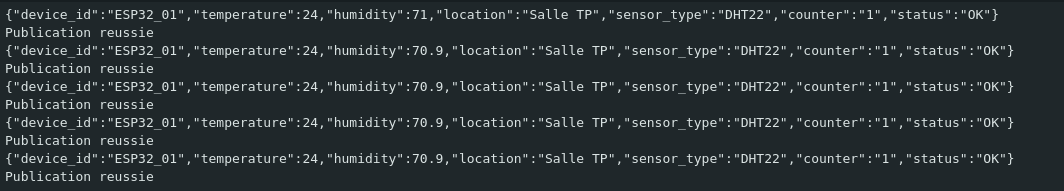
\includegraphics[width=0.88\textwidth]{serial.png}
\caption{Moniteur série de l'ESP32 : mesures publiées toutes les 5 secondes.}
\label{fig:serial}
\end{figure}

\begin{figure}[H]
\centering
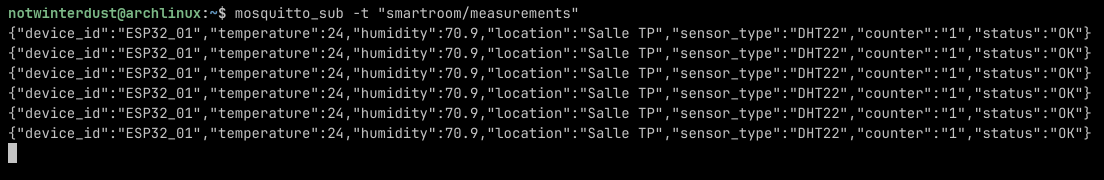
\includegraphics[width=0.88\textwidth]{console.png}
\caption{Réception des mesures par \code{mosquitto_sub} sur le topic \code{smartroom/measurements}.}
\label{fig:sub}
\end{figure}

\begin{figure}[H]
\centering
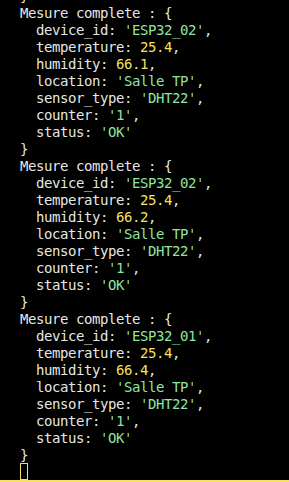
\includegraphics[width=0.48\textwidth]{server.png}
\caption{Console du serveur Node.js : mesures reçues des deux ESP32.}
\label{fig:node}
\end{figure}

\subsection{Scénarios de test}

\begin{table}[H]
\centering
\small
\begin{tabularx}{\linewidth}{@{}>{\bfseries}Y Y l@{}}
\toprule
Scénario & Résultat attendu & Statut \\
\midrule
Mesure périodique & JSON publié toutes les 5 s sur 4 topics & Observé (fig.~\ref{fig:serial}) \\
Abonné indépendant & \code{mosquitto_sub} reçoit les messages & Observé (fig.~\ref{fig:sub}) \\
Deux nœuds, réception serveur & « Mesure complete » pour chaque \code{device_id} & Observé (fig.~\ref{fig:node}) \\
Température $> 30\degC$ & alerte publiée, journalisée, affichée & À réaliser \\
Mesure hors plage / JSON invalide & « Mesure invalide », rien de diffusé & À réaliser \\
Coupure Wi-Fi / broker & reconnexion automatique du nœud & À réaliser \\
\bottomrule
\end{tabularx}
\caption{Scénarios de test et état de validation.}
\label{tab:scenarios}
\end{table}

% ---------------------------------------------------------------------------
\section{Analyse critique et pistes d'amélioration}
% ---------------------------------------------------------------------------

\subsection{Anomalies identifiées}
\label{sec:anomalies}

\begin{table}[H]
\centering
\small
\begin{tabularx}{\linewidth}{@{}>{\bfseries}c l Y Y@{}}
\toprule
N° & Fichier & Constat et conséquence & Correction proposée \\
\midrule
1 & dashboard.html & Marqueurs de conflit Git non résolus (lignes 71, 150 et 155). Erreur de syntaxe bloquante sur le script client. & Résoudre le conflit et harmoniser le script. \\
2 & esp2.c & Identifiant client MQTT \code{"ESP32_01"} identique à \code{main.c}. Provoque des déconnexions en boucle. & Utiliser \code{client.connect("ESP32_02")}. \\
3 & esp2.c & Le message d'alerte porte \code{device_id = "ESP32_01"}. & Corriger vers \code{"ESP32_02"}. \\
4 & main.c / esp2.c & Le champ \code{counter} vaut toujours la chaîne \code{"1"}. & Entier incrémenté à chaque envoi. \\
5 & package.json & Dépendance \code{socketio} obsolète/inutile. & Nettoyer avec \code{npm uninstall socketio}. \\
\bottomrule
\end{tabularx}
\caption{Anomalies relevées dans les scripts.}
\label{tab:anomalies}
\end{table}

\subsection{Pistes d'amélioration}

\begin{itemize}
  \item \textbf{Factorisation :} Regrouper les firmwares avec des constantes de configuration.
  \item \textbf{Hiérarchie des topics :} Adopter des topics dédiés par équipement (\code{smartroom/<device_id>/...}) avec des payloads optimisés.
  \item \textbf{Gestion des états :} Intégrer les messages « Last Will and Testament » (LWT) pour détecter la déconnexion inopinée d'un nœud.
  \item \textbf{Persistance :} Mémoriser l'historique dans une base de données (SQLite/InfluxDB) pour l'affichage de courbes temporelles.
\end{itemize}


\appendix

\end{document}